\documentclass[ngerman]{article}

% Packages
\usepackage[utf8]{inputenc}
\usepackage[german]{babel}
\usepackage{csquotes}
\MakeOuterQuote{"}

\usepackage[left=3cm,right=3cm,top=3cm,bottom=3cm]{geometry}
\usepackage[style=ieee]{biblatex}
\usepackage{amsmath}
\usepackage{amssymb}
\usepackage{graphicx}
\usepackage{hyperref}
\usepackage{titling}
\usepackage{caption}
\usepackage{listings}
\lstset
{
    basicstyle=\footnotesize,
    numbers=left,
    stepnumber=1,
    showstringspaces=false,
    tabsize=1,
    breaklines=true,
    breakatwhitespace=false,
    xleftmargin=.3\textwidth
}

\addbibresource{literatur.bib}

\newcommand{\subtitle}[1]{
  \posttitle{
    \par\end{center}
    \begin{center}\large#1\end{center}
    \vskip0.5em}%
}

\newcommand{\doublelinebreak}{\par\vspace{\baselineskip}}

\title{Implementierung eines ,,transformierenden" Interpreters für eine rudimentäre Programmiersprache auf Basis des untypisierten Lambda-Kalküls unter Verwendung von De-Bruijn-Indizes}
\author{Marvin Mielchen}
\subtitle{Hausarbeit aus dem Seminar: Grundlagen und Meilensteine der funktionalen Programmierung}
\date{\today}

\begin{document}

\maketitle

%\cite[S. 8]{nystrom}
- es muss einen Teil in der Arbeit geben der sich mit den Limitierungen der Arbeit beschäftigt
    - probleme mit rekusion in lambo
    - probleme mit speicher in lambo: z.B. sind while schleifen über große arrays wahrscheinlich nicht möglich weil alle expressions ausgewertet werden müssen und
    das also nicht "echt" iterativ ist
    - usw.
- DER Lambda Kalkül (üpberall ausbessern)

\section{Einleitung}

\subsection{Hintergrund und Motivation}

Im Jahr 1936 veröffentlichte Alonzo Church seine Arbeit (AUSFÜLLEN!!!) in der er den Lambda-Kalkül einführte. 
Der Lambda-Kalkül ist eine formale Sprache, die zur Untersuchung von Funktionen und deren Auswertung dient. Er ist die Grundlage der funktionalen Programmierung und hat einen großen Einfluss auf die Entwicklung von Programmiersprachen wie Lisp, ML, Haskell und vielen anderen.
Mit dem Lambda-Kalkül gibt es neben dem gängigen Modell der Turingmaschine ein weiteres Modell der Berechenbarkeit. Alle Berechnungen, die mit einer Turingmaschine durchgeführt werden können, können auch mit dem Lambda-Kalkül durchgeführt werden und umgekehrt.
Gleichzeitig entsprechen die Probleme die von Turingmaschinen gelöst werden können genau den intuitiv berechenbaren Problemen und das gilt so also auch für die Probleme, die mit dem Lambda-Kalkül modeliert werden können.
Der Lambda-Kalkül ist also ein universelles Modell der Berechenbarkeit und ist damit ein wichtiger Bestandteil der theoretischen Informatik. Viele Funktionale Sprachen werden auf den Grundlagen des Lambda Kalküls aufgebaut obwol unsere modernen Rechner mit ihrer von Neuman Architektur (CITE!) eher zu dem Modell der Turingmaschine passen.
Wie ein komplex verschachtelter Lambda Ausdruck mit einem imperativen System ausgewertet werden kann ist also eine interressante und komplizierte Problemstellung und soll die Motivation für diese Arbeit sein.

\subsection{Ziel der Hausarbeit}

- es soll auf der basis des untypisierten lambda Kalküls eine Sprache entwickelt werden die turingvollstäding (wenn auch nicht praktisch ist)
    - es werden also nur die allernötigsten features implementiert und entscheidende Eigenschaften einer "nützlichen" Sprache gegen Funktionalität eingetauscht die eine einfache und verständliche Interaktion mit den Regeln des Lambda Kalküls ermöglichen
- es soll ein Tree-Walk Interpreter entwickelt werden der die Sprache auswertet und dabei grundlegenden Anforderungen an einen modernen Interpreter und Ansprüchen an solche Implementationen zumindest im Ansatz gerecht wird 
- (optional) villeicht noch evaluation in irgendeiner form und vergleich mit anderen Sprachen 
- auch limitierungen der implementation betrachten (die sind schon schwerwiegend)

- im Anhang kann noch auf die Website eingegangen werden die eine Interaktion mit der entwickelten Sprache ermöglicht

\subsection{Übersicht über die folgenden Abschnitte}

\section{Grundlagen}

Für die Implementation des Interpreters werden einige Grundlagen benötigt die in den folgenden Abschnitten erläutert werden sollen.

\subsection{Syntax und Regeln im untypisierten Lambda-Kalkül !!ZITATE!!}

Der untypisierte Lambda-Kalkül beschreibt eine formale Sprache, die zur Definition und Analyse von Funktionen verwendet wird und dieselbe Klasse von berechenbaren Funktionen definiert wie die Turing-Maschine.
In der einfachsten Form lässt sich diese Sprache wie folgt rekursiv in Bakus Naur Form definieren:
\begin{align*}
    \text{\textless term\textgreater} & ::= \text{\textless variable\textgreater} \\
                      & \; | \; ( \lambda \text{\textless variable\textgreater} . \text{\textless term\textgreater} )\\
                      & \; | \; (\text{\textless term\textgreater} \; \text{\textless term\textgreater})
\end{align*}
Ein Lambda Term is dabei in einer der drei definierten Formen, wobei diese wiederum aus verschachtelten Lambda Termen bestehen können.

Eine Variable $\text{\textless variable\textgreater}$ kann im Lambda-Lalkül eine beliebige Zeichenketten sein (z.B. "x" oder "supervar") soweit keine der folgenden Zeichen enthalten ist: $\lambda$ . ( ). Variablen werden dabei als Platzhalter für beliebige Lambda Terme verwendet oder als formale Parameter von Abstraktionen und können dabei auch mehrfach in einem Lambda Term vorkommen.

$(\lambda \text{\textless variable\textgreater} . \text{\textless term\textgreater})$ heist Abstraktion und representiert eine Funktion. Die Variable ist dabei der formale Funktionsparameter und der Lambda Term nach dem Punkt ist der Funktionskörper. Ein Beispiel für eine Abstraktion ist die Identitätsfunktion $(\lambda x.x)$ welche ein Argument entgegennimmt und dieses unverändert zurückgibt.

$(\text{\textless term\textgreater} \; \text{\textless term\textgreater})$ heist Applikation und representiert den Aufruf einer Funktion. Der erste Lambda Term ist dabei die Funktion und der zweite Lambda Term ist das Argument. Die Applikation wird dabei von links nach rechts ausgewertet. Der erste Lambda Term muss aber nicht unbedingt eine Abstraktion sein. Er kann auch eine Variable oder eine Applikation sein. In diesem Fall wird der zweite Lambda Term als Argument an den ersten Lambda Term übergeben. Ein Beispiel für eine Applikation ist $((\lambda x.x) \; y)$ welches die Identitätsfunktion mit dem Argument $y$ aufruft und dabei $y$ zurückgibt.

\doublelinebreak
Um die Notation zu vereinfachen gibt es einige Konventionen die in der Literatur verwendet werden.
Zunächst soll Applikation linksassoziativ sein, d.h. $(t_1 \; t_2 \; t_3)$ soll als $((t_1 \; t_2) \; t_3)$ interpretiert werden. Bei einer langen Applikation werden also immer die ersten beiden Terme zuerst ausgewertet und das Ergebnis dann mit dem nächsten Term verknüpft. Die Abstraktion hingegen bindet immer so weit wie möglich nach Rechts. $(\lambda x.x \; x)$ wird also nicht als Applikation von $(\lambda x.x)$ auf $x$ interpretiert sondern als Abstraktion von $x$ auf $(x \; x)$. Mit explizieter Klammerung wird der Lambda Term also als $(\lambda x.(x \; x))$ geschrieben. Mit diesen Vereinfachungen kann ein komplexer Lambda Term wie
\begin{align*}
    (\lambda x.(\lambda y.(\lambda z.((x \; z) \; (y \; z)))))
\end{align*}
mit der folgenden Schreibweise dargestellt werden:
\begin{align*}
    (\lambda x. \lambda y. \lambda z. x \; z \; (y \; z)).
\end{align*}

\doublelinebreak

Ein sinvoller Äquivalenzbegriff für Lambda Terme ist die $\alpha$-Äquivalenz. Zwei Lambda Terme sind genau dann $\alpha$-Äquivalent, wenn sie sich nur in der Wahl der Variablennamen unterscheiden. Die folgenden Terme sind also $\alpha$-Äquivalent: $(\lambda x.x)$ und $(\lambda y.y)$.
Als $\alpha$-Konversion (geschrieben $\rightarrow_\alpha$) wird die Umbenennung von Variablen bezeichnet. Dabei wird eine Variable in einem Lambda Term durch eine andere Variable ersetzt wobei dabei keine freien Variablen gebunden werden dürfen. Zwei Terme sind auch genau dann $\alpha$-Äquivalent, wenn sie durch $\alpha$-Konversion ineinander überführt werden können.

\doublelinebreak

%Beta-Reduktion
Die Auswertung von Lambda Termen wird durch die $\beta$-Reduktion (geschrieben $\rightarrow_\beta$) beschrieben.
Dabei wird eine Applikation $((\lambda x.t_1) \; t_2)$ durch die Substitution von $t_2$ für $x$ in $t_1$ ersetzt. Die Substitution wird dabei so durchgeführt, dass keine freien Variablen gebunden werden. Die folgenden Beispiele sollen diesen Zusammenhang verdeutlichen:
\begin{align*}
    ((\lambda x.x) \; y)
\end{align*}
kann direkt durch die Substitution von $y$ für $x$ in $(\lambda x.x)$ ersetzt werden. Da in diesem Fall keine freien Variablen gebunden wird, kann die Substitution direkt durchgeführt werden und die Reduktion ergibt
\begin{align*}
    ((\lambda x.x) \; y) \rightarrow_\beta y.
\end{align*}
Das folgende Beispiel ist etwas komplexer:
\begin{align*}
    ((\lambda x.\lambda y.x \; y) \; y)
\end{align*}
Hier wird $y$ für $x$ in $\lambda y.x \; y$ substituiert. Da $y$ in $\lambda y.x \; y$ vorkommt, muss $y$ in $\lambda y.x \; y$ umbenannt werden damit das freie $y$ nicht gebunden wird. Es ergibt sich also
\begin{align*}
    ((\lambda x.\lambda y.x \; y) \; y) \rightarrow_\alpha ((\lambda x.\lambda z.x \; z) \; y) \rightarrow_\beta (\lambda z.y \; z).
\end{align*}

\doublelinebreak
Das sind alle Regeln die für den untypisierten Lambda-Kalkül benötigt werden. Mit diesen Regeln können alle berechenbaren Funktionen beschrieben werden wie sie auch mit einer Turingmaschine modeliert werden können.
Allerdings soll jetzt noch auf die De-Bruijn-Indizes eingegangen werden, die eine alternative Darstellung von Lambda Termen ermöglichen und die Implementierung eines Interpreters vereinfachen.

\subsection{De-Bruijn-Indizes}

Für die eben diskutierte $\beta$-Reduktion und die $\alpha$-Konversion gibt es einen entscheidenden Vorgang der sich für einen allgemeinen Lambda Term als schwierig erweist.
Bei beiden Äquivalentumformungen dürfen keine freien Variabeln gebunden werden und deshalb müssen kollidierende Variablen gefunden und umbenannt werden.
De-Bruijn-Indizes sind eine alternative Darstellung von Lambda Termen, bei denen dieses Problem deutlich vereinfacht wird weil die Variablen hier nicht mithilfe von Namen sondern mithilfe von Indizes identifiziert werden die nur von der Struktur des Lambda Terms abhängen.

Für einen Lambda Term in der Notation mit De-Bruijn Indizes verändert sich die Definition der Syntax wie folgt:
\begin{align*}
    \text{\textless term\textgreater} & ::= \text{\textless index\textgreater} \\
                      & \; | \; ( \lambda \text{\textless term\textgreater} )\\
                      & \; | \; (\text{\textless term\textgreater} \; \text{\textless term\textgreater})
\end{align*}
Ein Lambda Term ist also entweder ein Index, eine Abstraktion oder eine Applikation. Ein Index ist dabei eine natürliche Zahl die angibt wie weit der nächste Binder entfernt ist. Ein Index $0$ steht dabei für den nächsten Binder, ein Index $1$ für den übernächsten Binder und so weiter. Die folgenden Beispiele sollen diese Notation verdeutlichen:
\begin{align*}
    (\lambda x.x), (\lambda y.y), (\lambda z.z), usw.
\end{align*}
werden mit De-Bruijn-Indizes zu
\begin{align*}
    (\lambda 1).
\end{align*}
Die Identitätsfunktion kann mit der herkömmlichen Notation auf beliebig viele Arten dargestellt werden aber mit De-Bruijn-Indizes gibt es nur eine Möglichkeit. Der Index $1$ steht dabei für den nächsten Binder, also für das $\lambda$ und bedeutet bei der Substitution dass diese Variable dann ersetzt wird wenn das erste bindende $\lambda$ entfernt wird. 
Betrachten wir nun noch den komplizierteren Term
\begin{align*}
    (\lambda z.((\lambda y.y) \; (\lambda x.x)) \; (\lambda x.z \; x)).
\end{align*}
Mit De-Bruijn-Indizes lässt sich dieser mit
\begin{align*}
    (\lambda ((\lambda 1) \; (\lambda 1)) \; (\lambda 2 \; 1))
\end{align*}
darstellen. Die gebundenen $y$, $x$ und $z$ werden dabei alle durch den Index $1$ dargestellt weil sie alle nur ein $\lambda$ von ihrem Binder entfernt sind. $z$ hingegen bekommt den Index $2$ weil es zwei $\lambda$ von seinem Binder entfernt ist.
Mit dieser Notation werden die Änderungen der Indizies bei der Substitution während einer $\beta$-Reduktion deutlich einfacher. Wenn in einer Applikation der Term $N$ in die Abstraktion $M$ eingesetzt wird, müssen die Indizes in $M$ und $N$ wie folgt angepasst werden:
\begin{enumerate}
    \item Finde die Instanzen der Variablen $n_1, n_2, ..., n_k$ in einer Abstraktion $M$ die durch das $\lambda$ in $(\lambda \; M)$ gebunden werden.
    \item Dekkrementiere die freien Variablen in $M$ um die entfernung des äußeren $\lambda$-Binders zu kompensieren.
    \item Ersetze $n_1, n_2, ..., n_k$ durch $N$ und inkrementiere die freien Variablen in $N$ um die Anzahl der $\lambda$-Binder die mit der Substitution in $M$ dazu kommen.
\end{enumerate}
Eine $\beta$-Reduktion mit De-Bruijn-Indizes könnte dann z.B. wie folgt aussehen:
\begin{align*}
    ((\lambda \lambda 2) \; (\lambda 1)) \rightarrow_\beta (\lambda\lambda 1).
\end{align*}

\subsection{Funktionsweise von Interpretern und Compilern}

Als nächstes ist es noch sinvoll einige Grundlagen über die Funktionsweise von Interpretern zu erläutern. 
Traditionell gibt es bei der Ausführung von Programmen auf einem Computer zwei prominente Ansätze. Bei einem Compiler, wie er z.B. für Systemsprachen wie C oder C++ üblicher weise verwendet wird, wird der schon fast natürlich sprachige Quellcode in eine Maschinensprache übersetzt. Diese Maschinensprache ist dann direkt ausführbar und kann vom Computer verstanden werden. Bei einem Interpreter hingegen wird der Quellcode nicht in eine Maschinensprache übersetzt sondern in eine Zwischensprache die dann vom Interpreter ausgeführt wird. Der Interpreter ist also ein Programm, das den Quellcode eines anderen Programms einliest und ausführt.

Blickt man allerdings hinter den Vorhang, so sind die Unterschiede zwischen einem Compiler und einem Interpreter nicht so groß wie es auf den ersten Blick scheint. Wie Robert Nystrom in seinem Buch "Crafting Interpreters" (CITE!) beschreibt, gibt es verschiedene Stufen der Analyse die sowohl bei einem Compiler als auch bei einem Interpreter durchgeführt werden müssen.

\begin{figure}
    \centering
    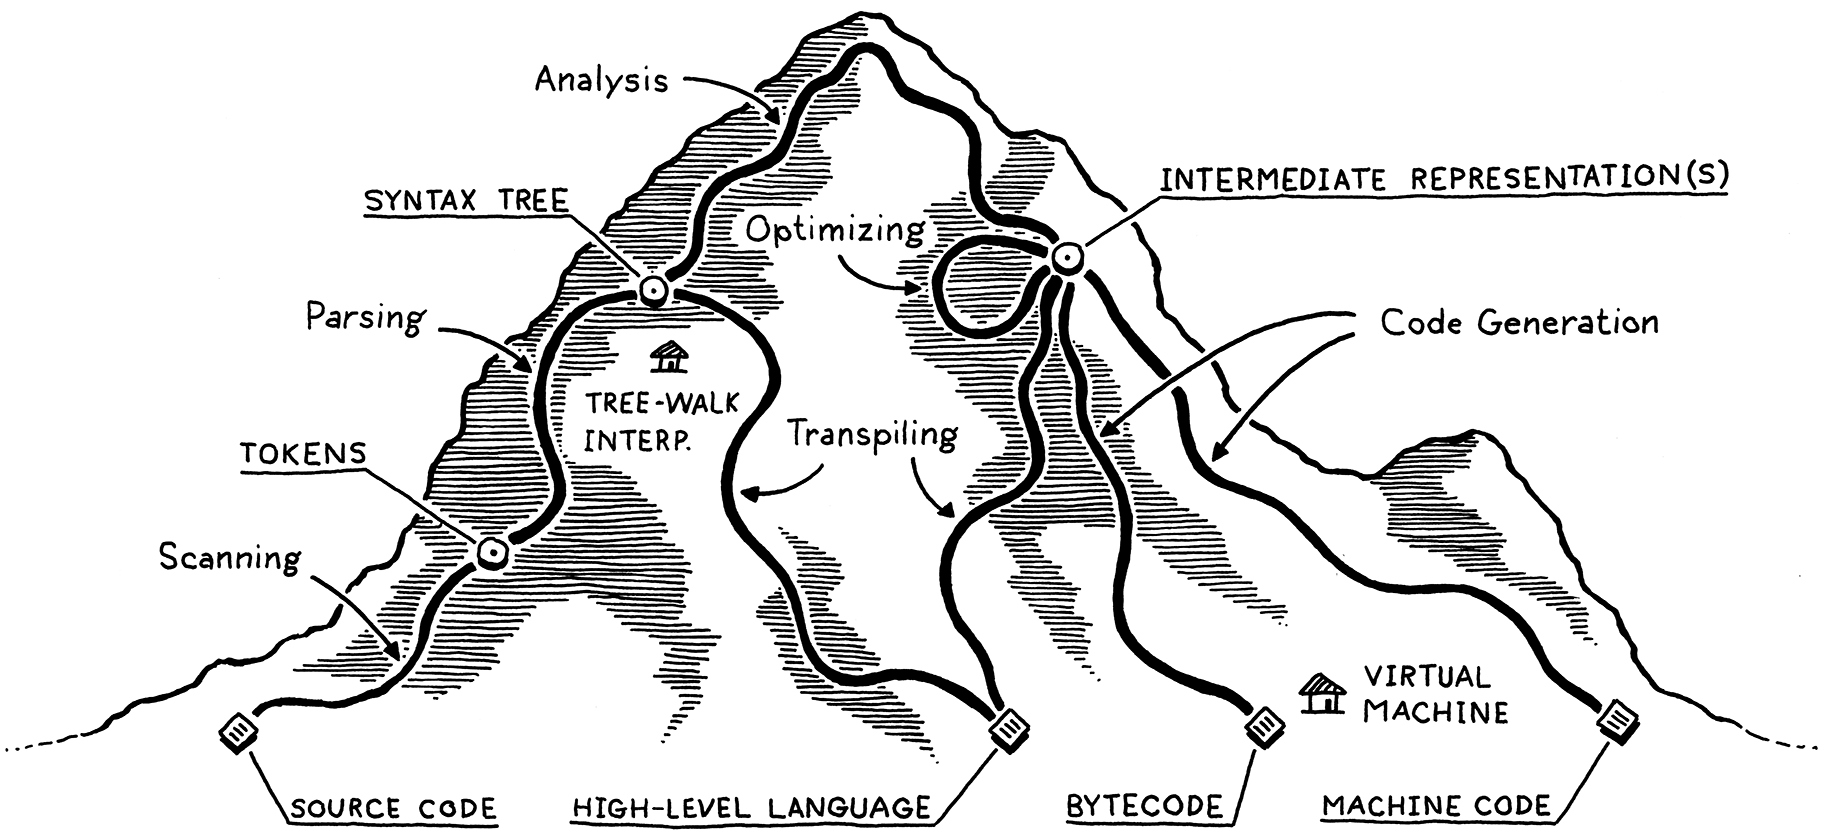
\includegraphics[width=0.8\textwidth]{mountain.png}
    \caption{Funktionsweise eines Interpreters ZITIEREN!!!}
    \label{fig:interpreter}
\end{figure}

Der erste Schritt ist die Lexikalische Analyse. Dabei wird der Quellcode in einzelne Tokens zerlegt. Ein Token ist dabei eine Zeichenkette die eine Bedeutung hat. Ein Token kann z.B. ein Schlüsselwort wie "if" oder "while" sein, eine Zahl oder eine Variable. Die Tokens werden dabei in einer Liste gespeichert und an den Parser weitergegeben.

Der Parser ist der nächste Schritt. Er nimmt die Liste von Tokens und baut daraus eine Datenstruktur auf. Diese Datenstruktur wird in der Literatur Syntax Baum (engl. Syntax Tree) oder Abtract Syntax Tree (AST) genannt. Ein AST ist eine Baumstruktur die den Quellcode repräsentiert. Die Knoten des Baums sind dabei die Operatoren und die Blätter sind die Operanden. Der Syntax Baum ist dabei eine abstrakte Repräsentation des Quellcodes und enthält keine Informationen über die Bedeutung der einzelnen Knoten. 

\doublelinebreak

Von hier aus gibt es nun verschiedenste Möglichkeiten wie der Syntax Baum weiter verarbeitet werden kann. Bei einem Compiler wird der Syntax Baum in eine Zwischensprache übersetzt und dann in Maschinencode. Bei einem Interpreter wird der Syntax Baum direkt ausgeführt. Es gibt aber auch noch andere Möglichkeiten. So kann der Syntax Baum z.B. in eine andere Sprache übersetzt werden oder in eine andere Form der Zwischensprache. Der Syntax Baum kann auch in eine andere Form der Zwischensprache übersetzt werden und dann von einem Interpreter ausgeführt werden. Es gibt also viele verschiedene Möglichkeiten wie ein Interpreter oder Compiler aufgebaut sein kann.

Bei modernen Interpretern gibt es z.B. das Konzept von Just-In-Time (JIT) Compilation. Dabei wird der Syntax Baum in eine Zwischensprache übersetzt und dann aber nicht direkt ausgeführt sondern in einem JIT Compiler in Maschinencode übersetzt. Dieser Maschinencode wird dann ausgeführt. Der Vorteil dieses Ansatzes ist, dass der JIT Compiler den Maschinencode optimieren kann und so die Ausführung beschleunigt werden kann. So arbeiten viele Interpreter intern trotzdem mit einem Compiler und Ausführung von Maschinencode.

Weiterer Erklärungsbedard besteht noch bei dem Begriff eines transformierenden Interpreters so wie er in dem Titel dieser Arbeit angekündigt wird. Im Rest der Arbeit soll eine Sprache entwickelt werden welche grundlegenden Regeln des Lambda Kalküls implementiert und so die Modellierung aller berechenbaren Funktionen ermöglicht. Dieser Interpreter soll Quellcode mit Lexikalischer Analyse und Parsing in einen Syntax Baum übersetzen, diesen Syntax Baum dann in eine Zwischenrepresentation (IR) übersetzen, Umformungen und berechungen durchführen und den Resultierenden AST dann wieder in die Ausgangssprache übersetzten. Der Interpreter soll also den Quellcode nicht komplett ausführen sondern nur in eine andere Form übersetzen. Damit handelt es sich nicht um einen traditionellen Interpreter sondern um ein System das eher einem Transpiler ähnelt - Transpiler übersetzen Programme von einer Sprache in eine andere. Der Begriff Interpreter soll hier aber trotzdem verwendet werden weil die Interaktion des Nutzers mit dem System eher der eines Interpreters als eines Transpilers ähnelt. hier werden tatsächlich berechnungen durchgeführt und es werden auch immer Teile des ASTs tatsächlich ausgewertet.

Daher wurde hier auch der unübliche Begriff eines transformierenden Interpreters gewählt, wobei das Transformieren für die Umformungen und Berechnungen steht die der Interpreter durchführt um dies Ausgabe zu erzeugen.

\section{Design und Implementierung des Interpreters}

- nachdem jetzt die Grundlagen geklärt sind kann es jetzt um die eigentliche Implementation gehen
- Sprache soll Lambo heißen (Lambda Online)

\subsection{Beschreibung der Programmiersprache Lambo}

Das Ziel dieser Arbeit ist sich die Implementation des Lambda Kalküls in einer Programmiersprache zu betrachten und dabei die grundlegenden Regeln des Lambda Kalküls zu implementieren. Da die Sprache so also keine starken Anforderungen an einen praktischen nutzen für besonders performante Berechungen oder generell an eine nützliche Programmiersprache stellt, können andere Konzepte und Eigenschaften in den Vordergrund gestellt werden, die normalerweise nicht zu einer gängigen Programmiersprache gehöhren und auch die Implementation vereinfachen.

Das Ziel soll eine Website mit einem Code Editor sein in dem man Quellcode eingeben kann und dann die verschachtelten Lambda Terme schritt für Schritt umformen und reduzieren kann (TODO: Screenshot). Dieser Auswertungsmechanismus ermöglicht nicht nur eine Leehrreiche Interaktion, für das verständlich machen der Regeln des Lambda Kalküls, sondern vereinfacht auch die Implementation des Interpreters wie sich später zeigen wird.

Weil die zu entwickelnde Sprache in einem Online Editor verwendet werden soll und nur auf den grundlagen des Lambda Kalküls basiert soll sie auch einen Namen bekommen der diese Eigenschaften widerspiegelt:
Daher wir die zu entwickelnde Sprache im folgenden Lambo (angelehnt an Lambda Online) genannt.


\subsubsection{Syntax und Semantic}

Wie im Lambda Kalkül soll es in der Sprache Lambo nur Funktionen geben. 
Um allerdings mehrere Funktionen in einem Programm modelieren zu können wird zusätzlich auch ein Statement für die Wertezuweisung benötigt. Dafür soll in Lambo das Schlüsselwort "def" verwendet werden. Außerdem soll statt der herkömlichen Notation mit $\lambda$ und . die Notation mit runden Klammern und geschweiften Klammern verwendet werden, da diese Notation für einen Qellcode sorgt der populären Programmiersprachen wie z.B. Python ähnelt.
Eine erste Skizze der Syntax von Lambo hat also die folgende Strucktur:
\begin{align*}
    \text{\textless lambo-programm\textgreater} & ::= \text{\textless statement\textgreater}* \\
    \text{\textless statement\textgreater} & ::= \text{\textless definition\textgreater} \\
    \text{\textless definition\textgreater} & ::= \text{def} \; \text{\textless variable\textgreater} \; \text{\textless expression\textgreater}\\
    \text{\textless expression\textgreater} & ::= \text{\textless variable\textgreater} \; | \; \text{\textless abstraction\textgreater} \; | \; \text{\textless application\textgreater}\\
    \text{\textless variable\textgreater} & ::= \text{\textless letter\textgreater +} \\
    \text{\textless abstraction\textgreater} & ::= (\text{\textless variable\textgreater})\{\text{\textless lambda-term\textgreater}\}\\
    \text{\textless application\textgreater} & ::= \{\text{\textless lambda-term\textgreater} \; \text{\textless lambda-term\textgreater}\} \\
    \text{\textless letter\textgreater} & ::= a \; | \; b \; | \; c \; | \; ... \; | \; z | \; A \; | \; B \; | \; C \; | \; ... \; | \; Z | \; 0 \; | \; 1 \; | \; 2 \; | \; ... \; | \; 9
\end{align*}
Die BNF zeigt die grundlegende Strucktur für ein Lambo Programm. Ein Lambo Programm besteht aus beliebig vielen Statements. Ein Statement wiederum ist eine Definition die mit dem Schlüsselwort "def" beginnt und einer Variable einen Lambda Ausdruck zuweist. Ein Lambda Ausdruck wiederum ist wie gewohnt entweder eine Variable, eine Abstraktion oder eine Applikation wobei die Syntax für die Lambda Ausdrücke hier ein Bisschen anderes gewählt ist als für das Lambda Kalkül üblich. Um diese Syntax verständlicher zu machen folgen nun einige Beispiele für Lambo Programme. \\ \\
Eine einfache Identitätsfunktion wie $(\lambda x.x)$ kann in Lambo wie folgt aussehen:
\begin{lstlisting}
def ifunc (x) {
    x
}
\end{lstlisting}
In Lambo muss aber jeder Ausrduckt eine Definition sein deshalb wird der Lambda Ausdruch hier dem Symbol "ifunc" zugewiesen. Gleichermaßen lässt sich auch eine Variable in Lambo definieren:
\begin{lstlisting}
def a b
\end{lstlisting}
Hier wird die Variable b dem Symbol "a" zugewiesen. Für eine Applikation geht das ganze dann so:
\begin{lstlisting}
def app {
    a b
}
\end{lstlisting}
Wieder ist eine Definition nötig um den Lambda Ausdurck in Lambo darzustellen. Hier wird die Aplikation von a auf b dem Symbol "app" zugewiesen. Auch verschachtelte Funktionen sind mit dieser Definition der Syntax möglich:
\begin{lstlisting}
def someapp {
    (x) {
        x
    }
    a
}
\end{lstlisting}
Hier wird someapp die Applikation der Identitätsfunktion auf a zugewiesen. 
Da unsere Syntax bereits mehrere Funktionen in einem Programm ermöglicht, ist es auch der folgende Quellcode ein gültiges Lambo Programm:
\begin{lstlisting}
def a b
def c d
def e f
\end{lstlisting}
\doublelinebreak
Damit lässt sich bereits alles modelieren was an berechnbaren Fukntionen möglich ist. Allerdings ist die Syntax noch nicht ganz vollständig. Es fehlt noch die Möglichkeit Funktionen mit mehreren Parametern zu definieren. Dafür soll in Lambo die Syntax für Abstraktionen erweitert werden. Die erweiterte Syntax für Abstraktionen sieht dann wie folgt aus:
\begin{align*}
    \text{\textless abstraction\textgreater} & ::= (\text{\textless variable\textgreater}*)\{\text{\textless lambda-term\textgreater}\}\\
\end{align*}
Damit sind nun auch Funktionen mit mehreren Parametern möglich z.B.:
\begin{lstlisting}
def func (x y) {
    x
}
\end{lstlisting}
Das entspricht dann der Funktion $(\lambda x.\lambda y.x)$ im Lambda Kalkül. Und kann in Lambo auch mit einstelligen Funktionen umgesetzt werden:
\begin{lstlisting}
def func (x) {
    (y) {
        x
    }
}
\end{lstlisting}
Dieses Konzept wird auch Currying genannt und ist eine wichtige Eigenschaft von Lambo. Currying bedeutet, dass eine Funktion mit mehreren Parametern in mehrere Funktionen mit jeweils einem Parameter umgewandelt wird. Die Funktion $(\lambda x.\lambda y.x)$ wird also in Lambo zu $(\lambda x.(\lambda y.x))$ umgewandelt. Das hat den Vorteil, dass Funktionen mit mehreren Parametern in Lambo nicht anders behandelt werden müssen als Funktionen mit nur einem Parameter. Das vereinfacht die Implementation des Interpreters und ist auch ein Grund warum die Syntax von Lambo so gewählt wurde wie sie ist. Um eine ähliche Vereinfachung auch für die Applikationen zu erreichen, soll in Lambo auch die Syntax für Applikationen erweitert werden. Die erweiterte Syntax für Applikationen sieht dann wie folgt aus:
\begin{align*}
    \text{\textless application\textgreater} & ::= \{\text{\textless lambda-term\textgreater} \; \text{\textless lambda-term\textgreater}*\} \\
\end{align*}
Damit wird die linksassoziativ der Applikation auch in Lambo übernommen und ermöglicht es so eineige Klammern einzusparen. Statt
\begin{lstlisting}
def app {
    {{a b} c}
}
\end{lstlisting}
kann in Lambo also auch
\begin{lstlisting}
def app {
    a b c
}
\end{lstlisting}
geschrieben werden. Damit ist die Syntax von Lambo bis auf Quelltext-Kommentare (TODO: siehe Anhang) vollständig.

\subsection{Implementierung des Interpreters}

\captionsetup{labelformat=empty}
\lstset{
    language=Java,
    frame=single,
    breaklines=true,
    numbers=left,
    stepnumber=1,
    showstringspaces=false,
    tabsize=1,
    breaklines=true,
    breakatwhitespace=false,
    xleftmargin=.1\textwidth,
    xrightmargin=.1\textwidth
}

Wie auch bei der ersten Implementationen eines Interpreters aus dem Buch von Nystrom (TODO: CITE!), soll auch hier der Interpreter mit Java implementiert werden. So müssen schwierige Probleme wie die Speicherverwaltung nicht beachtet werden und das Lambda Kalkül steht im Fokus. Außerdem lässt sich für den Lambo Interpreter in Java später leicht mit vorhandenen Java Bibliotheken eine funktionstüchtige HTTP API umsetzen.

Im folgenden werden die einzelnen Komponenten des Interpreters vorgestellt und die Implementation erläutert. Dabei wird allerdings auf den vollständigen Quellcode verzichtet und nur vereinfachte Quelltext-Ausschnitte der wichtigsten Teile der Implementation vorgestellt. Unter den Codebeispielen werden die Zeilennummern der jeweiligen vollständigen Quelltext Datei angegeben die im Anhang zu finden sind.

\subsubsection{Lexer}

Zunächst muss der Quelltext mit einem Lexer in einzelne Tokens zerlegt werden. Dafür braucht es eine Klasse für die Tokens:
\begin{lstlisting}[caption={TODO: Referenz zu Anhang}, captionpos=b]
public class Token {
    public final TokenType type;
    public final String lexeme;
}
\end{lstlisting}
Ein Token hat dabei einen Typ und ein Lexeme welches den Inhalt des Tokens repräsentiert. Der Typ des Tokens wird dabei durch eine Enumeration definiert:
\begin{lstlisting}[caption={TODO: Referenz zu Anhang}, captionpos=b]
public enum TokenType {
    LEFT_PAREN, RIGHT_PAREN, LEFT_BRACE, RIGHT_BRACE, SEMICOLON, EQUAL,
    IDENTIFIER,
    DEF,
    EOF
}
\end{lstlisting}
Jeder Token in der Sprache Lambo lässt sich also genau einem Typ zuordnen. Ein Token kann dabei ein Sonderzeichen wie "(" oder ")" sein, ein Schlüsselwort wie "def" oder eine Variable. Die Variable wird dabei durch den Typ "IDENTIFIER" repräsentiert und das Lexeme der Variable ist dann der Name der Variable.



\subsubsection{Parser}

currying muss rein irgendwo

\subsubsection{De-Bruijn-Indizes}

\subsubsection{interpreter}

\section{Evaluation und Tests}

\subsection{Konstruktion von Natürlichen Zahlen, Boolean Artimethik und Listen}

\subsection{Herausforderungen und Lösungen - Limitierungen der Implementation}

\subsection{Performance-Analyse des Interpreters}

\subsection{Vergleich mit anderen Interpretern}


\section{Zusammenfassung, Fazit und Ausblick}

\subsection{Mögliche Anwendungen von Lambo}

\subsection{Potenzielle Erweiterungen des Interpreters}

\subsection{Zukünftige Entwicklungsrichtungen}

\subsection{Zusammenfassung der Ergebnisse}

\subsection{Schlussfolgerungen und Ausblick}

%\printbibliography
\end{document}
